% % % Set the style for this file:
\pagestyle{standard}

% % % Beginning of the chapter
\chapter{Results and discussion}\label{chapter4}

	% % % Set the style for the first page:
	\thispagestyle{chapter-first-page}

	\section{Petal thermal cycles.}\label{section4.1}
	
		For both thermal cycles the set points were selected by varying the $CO_{2}$ pressure (See Table \ref{tab2.2}) in such a way that we go from room temperature to the lowest possible temperature and back in steps of 5\space$^\circ C$. Then, all the data from PT100, SHT21 and TRACI sensors in addition to the power supply outputs is recorded at each set point. Also, the Petal thermograms are recorded following the method described in section \ref{section2.2} at each step. The results are shown in Figure \ref{fig4.1} for both cycles 2 (top) and 9 (bottom). Uncertainties of the IR measurements have not been included not to overload the plots but, as discussed also in Section \ref{section2.2}, the main source of uncertainty comes from the IR camera itself. In total, uncertainties on the black tape measurements are between (2 - 2.5) \%.
		
		\begin{figure}[ht!]
			\centering
			\captionsetup{justification=centering,margin=0cm}
			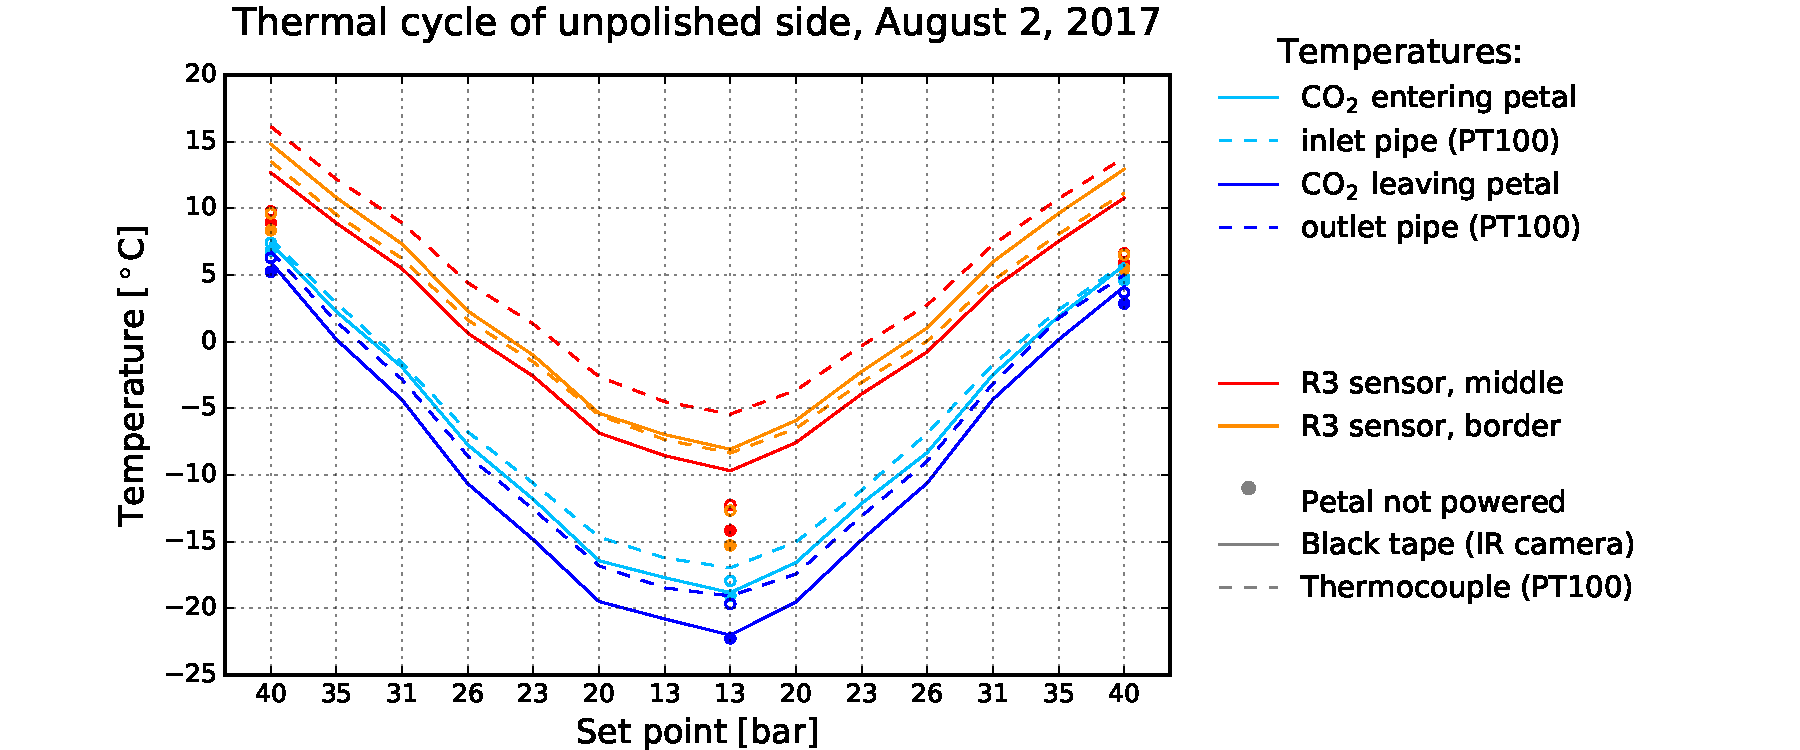
\includegraphics[scale=0.45]{Figures/Chapter04/unwrapped_cycle_2_201711121522.pdf}
			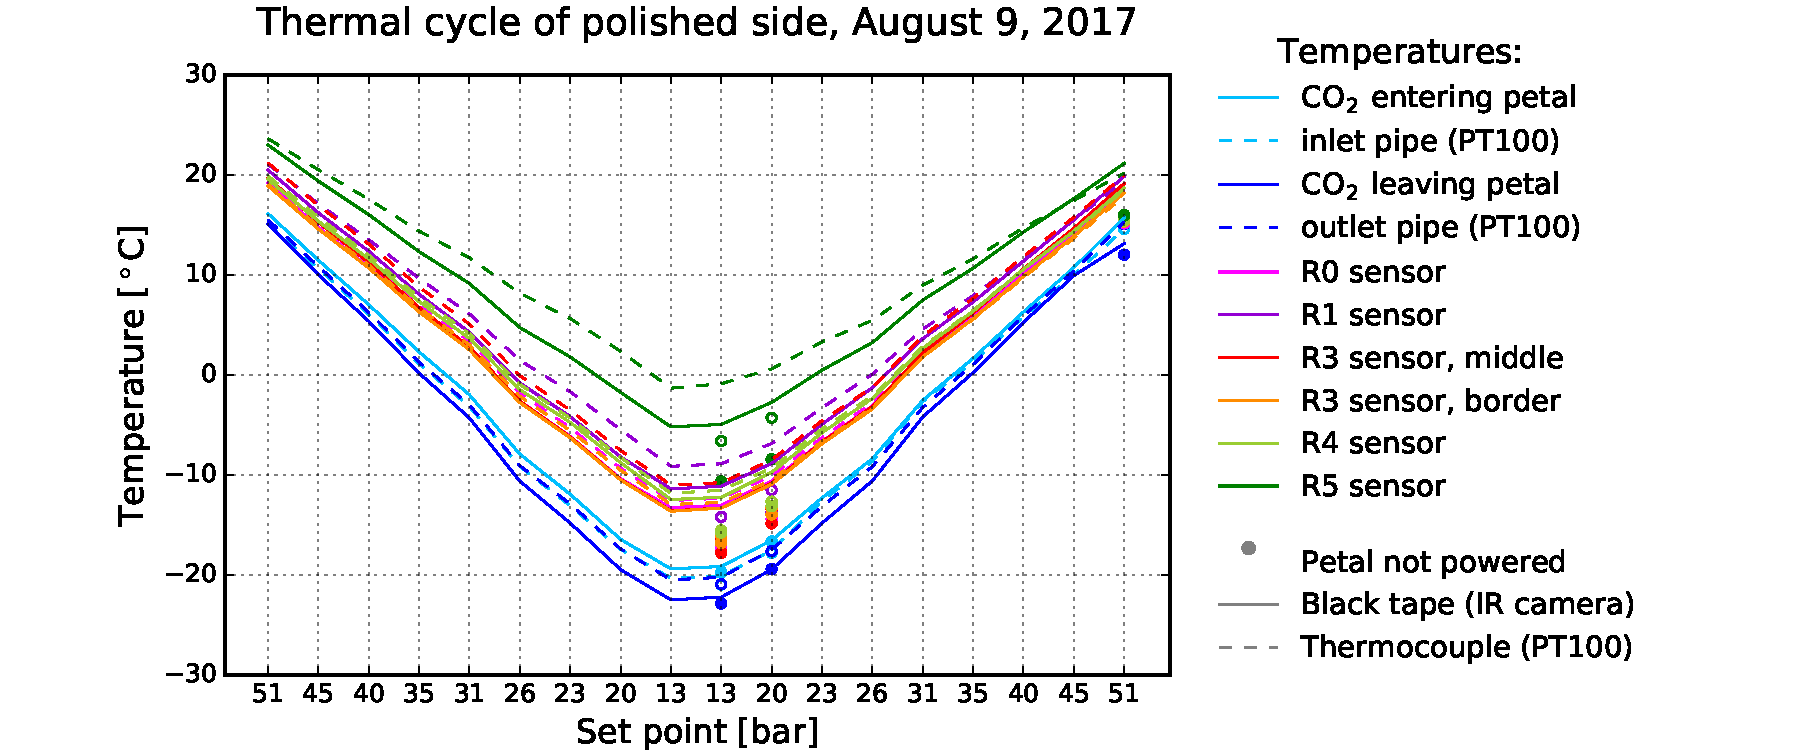
\includegraphics[scale=0.45]{Figures/Chapter04/unwrapped_cycle_9_201711121522.pdf}
			\caption{Temperature plots for the thermal cycles 2 (top) and 9 (bottom). The dots represent set points with the Petal not powered and the lines correspond to set points with both sides of the Petal powered. Solid lines and filled dots represent black tape readings with the IR camera (except CO2 entering/leaving petal) and dashed lines and hollow dots represent thermocouple values.}\label{fig4.1}
		\end{figure}	
		
		As it can be seen, with cycle 2 we were able to reach temperatures of around -18\space$^\circ C$ and -20\space$^\circ C$ with cycle 9. For both cycles it is also notable the fact that the returning $CO_{2}$ is colder which is consistent with dual-phase cooling. We can also see that the PT100 thermocouple sensors report consistently higher temperatures that the TRACI sensors for both inlet and outlet pipes  meaning that we either lose some cooling power due to thermal conductivity of the pipes, which is expected, or one of the sensors is incorrectly calibrated/placed. This situation is the opposite in cycle 9 with the inlet fluid temperature readings. In fact, for cycle 9, the inlet PT100 accidentally broke and had to be re-glued which might explain the difference from one cycle to the other in the inlet pipe while the outlet remained somewhat the same. This indicates that a correct manipulation of the sensors is crucial to obtain good reliability on the measurements.
		Another interesting test that we wanted to perform was the comparison between the temperature reported by the IR camera using the black tape method and the temperature measured with an alternative method on the same surface (e.g. using PT100 thermocouples). In order to perform such a test, the additional PT100 sensors placed on the silicon surface were hold in position using the same high emissivity black tape used for the strips of the “Zebra” Petal. For cycle 2 only two PT100s were used, as described in Chapter 2 while for cycle 9 four additional ones were placed. From Figure \ref{fig4.1} (top) we can see that the readings of the thermocouple and the IR camera are quite different for the sensor placed between the ASICs, possibly due to miss-contact with the silicon surface (the sensors had to be placed very carefully not to damage the silicon). The other PT100 sensor, on the other hand, shows relatively good agreement with the IR camera measurement. The situation in cycle 9 improved a bit more, in general, for the lowest setpoint, specially in the R0, R3(border) and R4, even though there are still large discrepancies (e.g. R5).
			
	
	\section{Comparison with FEA results.}\label{section4.2}
	
		In order to compare the results with FEA simulations, the IR camera temperature measurements from ROI markers on the surface of the black tape strips was used. Figure \ref{fig4.2} shows the lowest point thermogram for cycle 2 where the tiny red squares are the IRBIS measurement markers. Using linear interpolation between the marker points we were able to produce a sort of isotherms map of the sensors as shown in figure \ref{fig4.3} (top). Figure \ref{fig4.3} (bottom) shows the FEA simulation results [15].
		
		\begin{figure}[ht!]
			\centering
			\captionsetup{justification=centering,margin=2cm}
			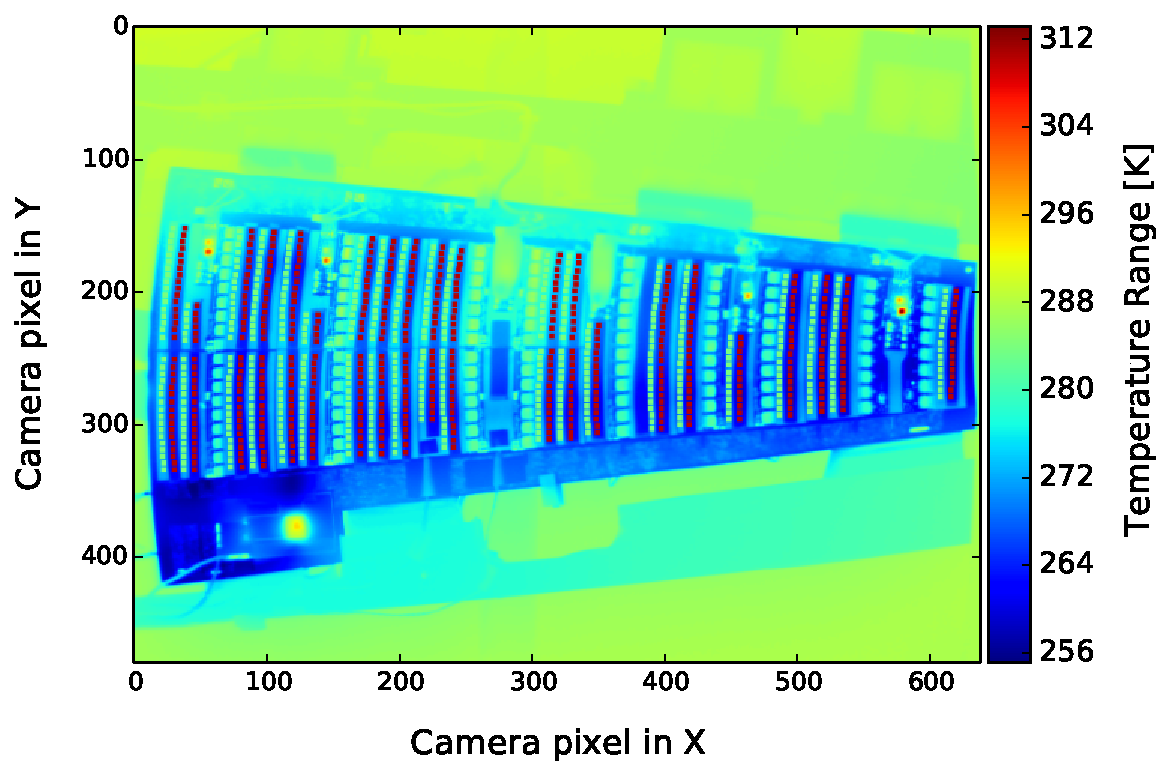
\includegraphics[scale=0.65]{Figures/Chapter04/thermo_Temp_20170803154926.pdf}
			\caption{Thermogram of the lowest setpoint in cycle 2 showing the IRBIS measurement areas (markers) defined on the black tape (red squares) and the corresponding silicon surface ones (blue squares).}\label{fig4.2}
		\end{figure}
		
		Before discussing the differences between the images in Figure \ref{fig4.3}, we must say that this is to some extent an unfair comparison. While in FEA one have access to virtually every temperature point we are limited by the number of markers and their uncertainty. Furthermore, the characteristics of the FEA model are not exactly compatible (e.g. power board thickness, cooling loop) and the very complicated convection/absorption with the air surrounding the Petal is very hard to model. In fact, we know that the values of temperature reported by the markers near the R3 electronics (hottest point) is greatly influenced by the “halo” surrounding it, as discussed in Chapter \ref{chapter2}. In addition, in that precise region of the image, the linear interpolation tries to figure out a large area where there is no experimental point and thus, this area should not be very well described.
		In general (without paying too much attention to the temperature magnitudes), some similar features can be found between the experimental results and the FEA model, specially to the left side of the Petal (R4 and R5).
		
		\begin{figure}[ht!]
			\centering
			\captionsetup{justification=centering,margin=0cm}
			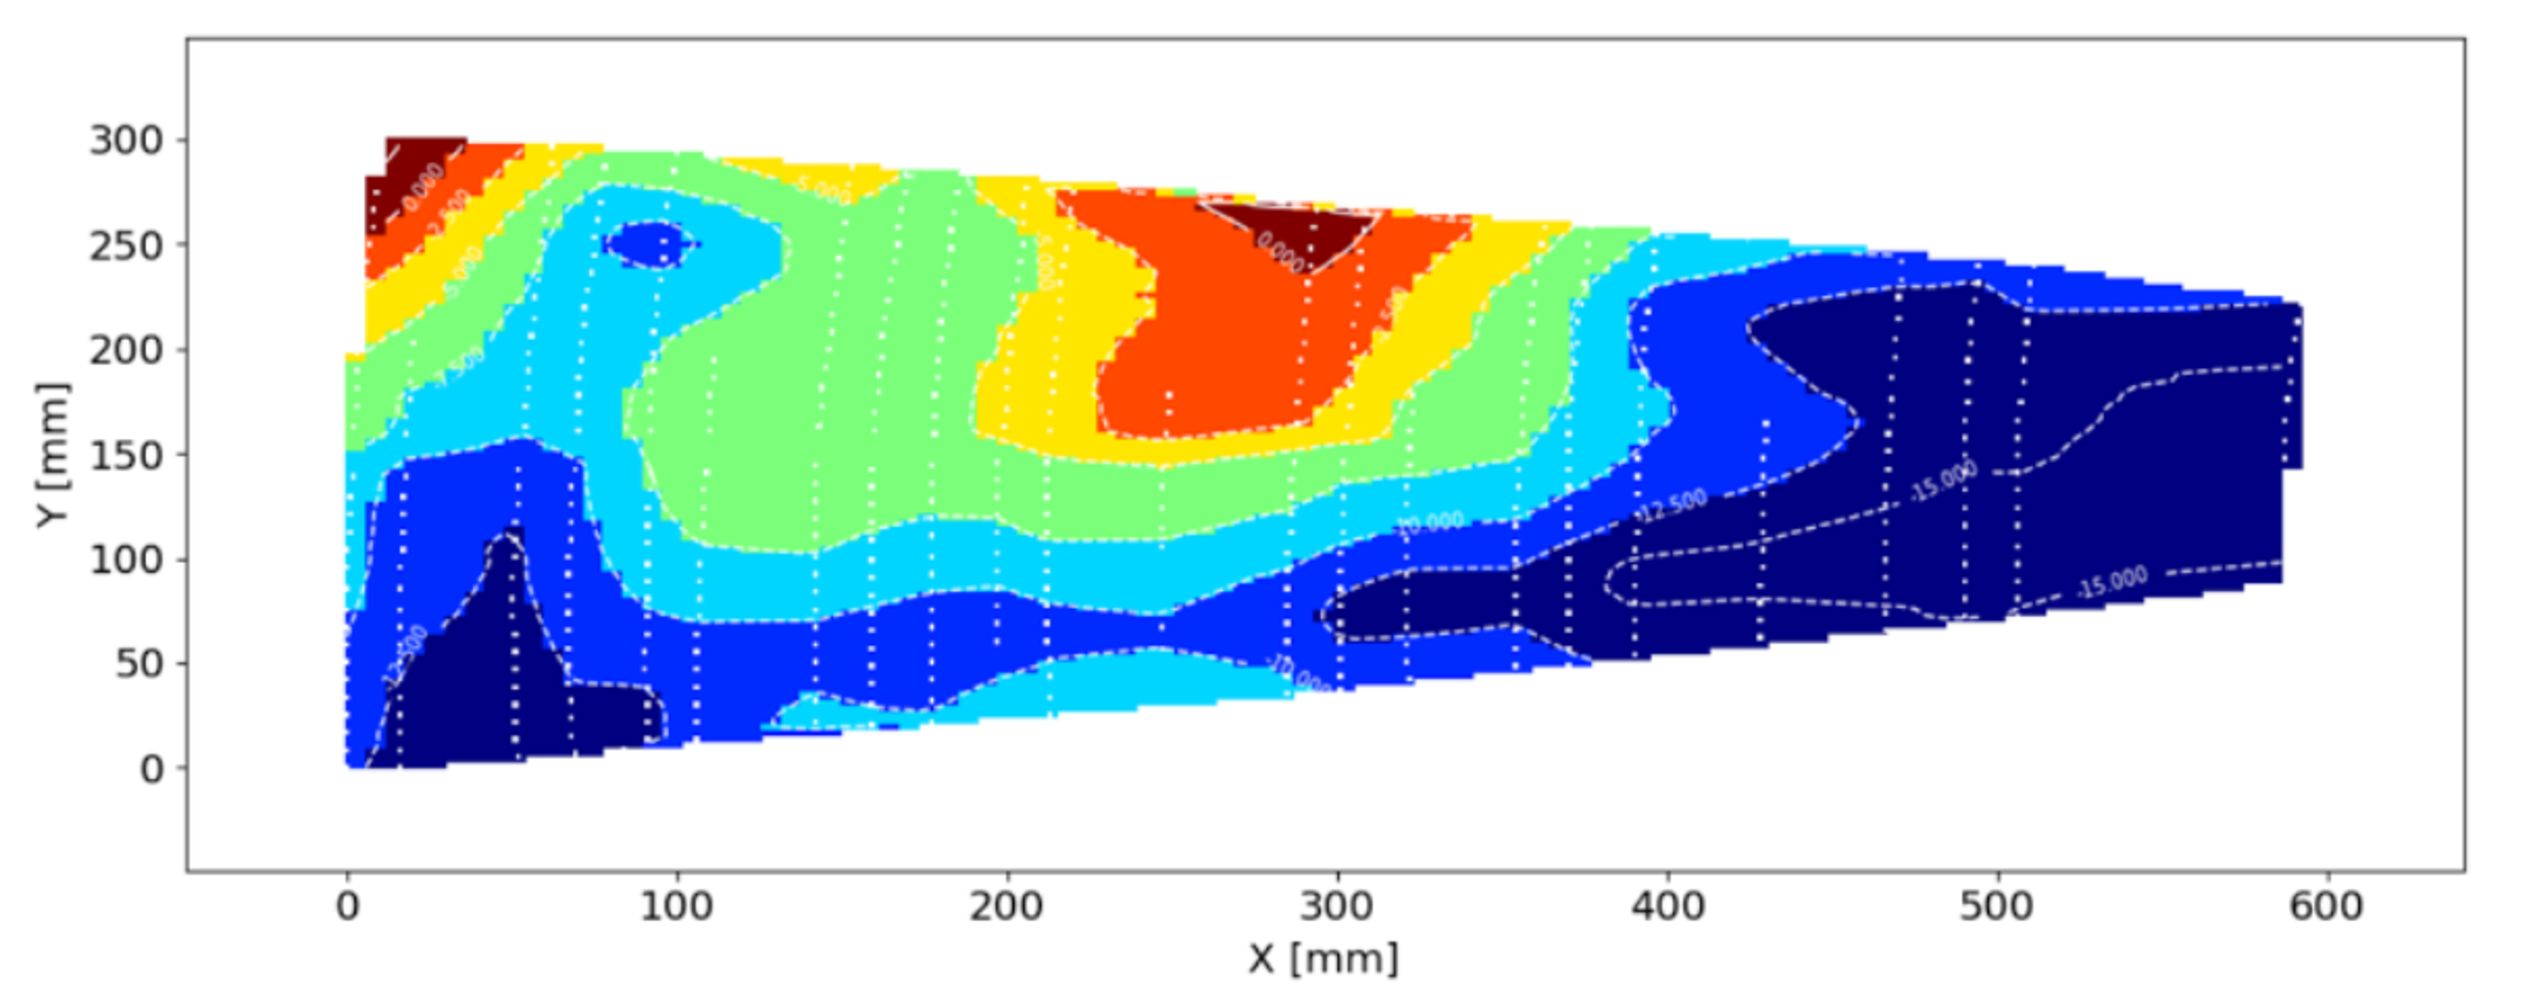
\includegraphics[scale=0.35]{Figures/Chapter04/PetalLinearInterpolation.pdf}
			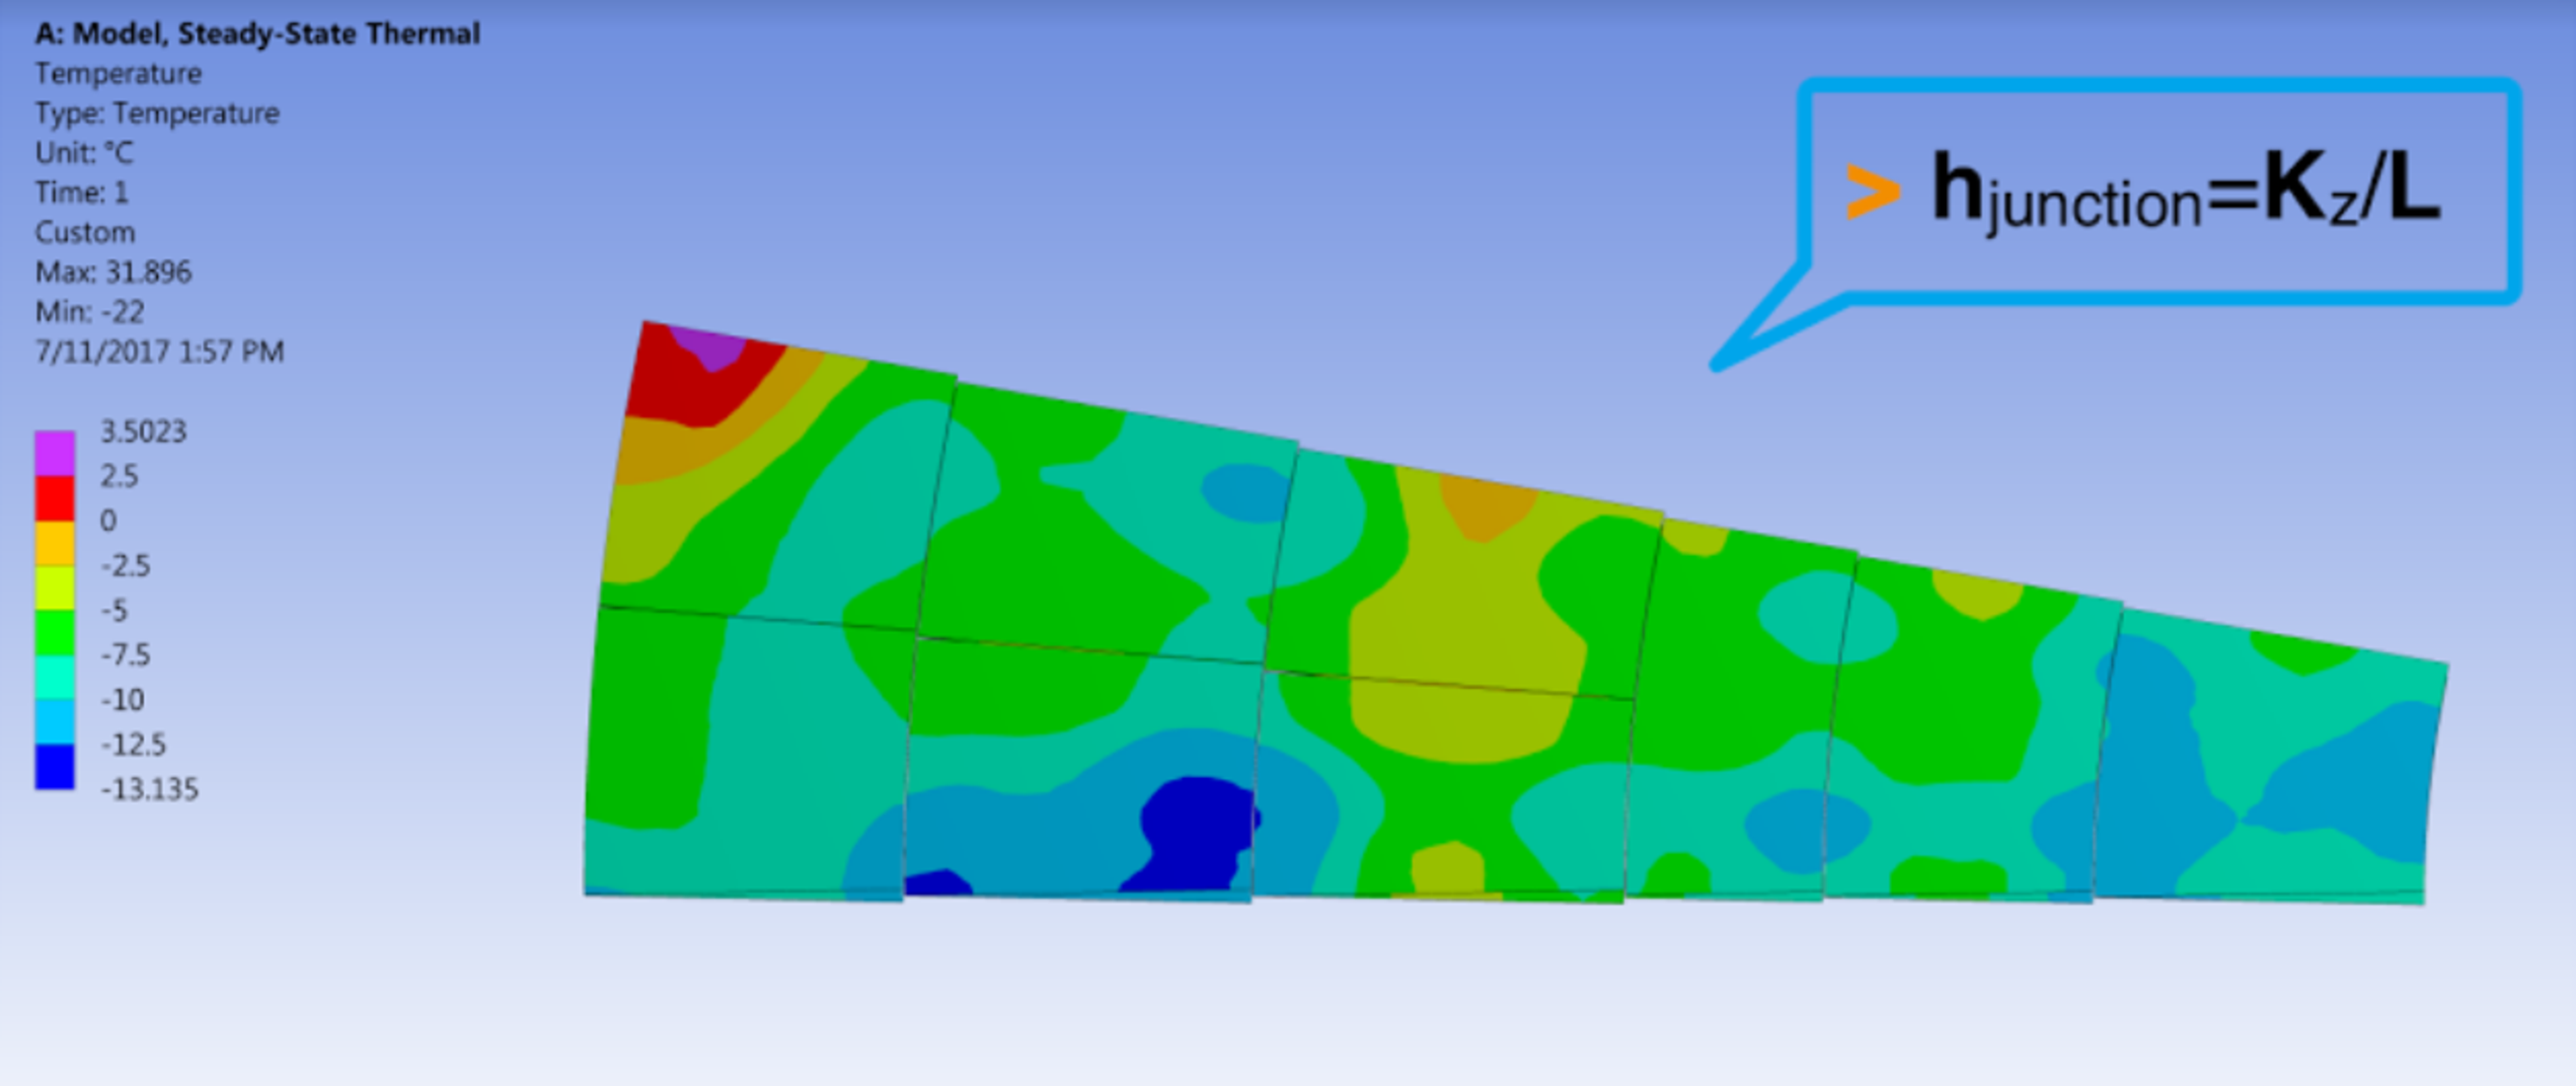
\includegraphics[scale=0.35]{Figures/Chapter04/PetalFEA.pdf}
			\caption{Temperature profiles for the silicon sensors of the unpolished side of the Petal. (Top): experimental IR measurements results. (Bottom): FEA simulation.}\label{fig4.3}
		\end{figure}
	
	\section{Silicon emissivity estimation.}\label{section4.3}
	
		As shown in the previous section, one of the factors affecting the robustness of the measurements is the lack of “resolution” by using the black tape method, even though more than 560 markers were created (by hand) on the surface of the silicon sensors. This asks for more refined ways to measure the temperature of the silicon sensors. Furthermore, the black tape method is a quite invasive technique to use with the current prototype and for sure something to avoid during quality control with real Petals.
		A good first approach would be to try to estimate the silicon emissivity and then use this value to correct globally the IR image. As mentioned in Chapter \ref{chapter3}, a relative method using the black tape markers measurements as temperature reference can be used to calculate the emissivity of the silicon next to them employing Equation \ref{eq3.14}. The IRBIS software also has an emissivity calculator which reports the emissivity of a given pixel if we provide the real temperature of the pixel and the ambient temperature (apparent reflected temperature). However, as this variant is more like a black box to us, we decided to use both methods and compare the results. As mentioned also in Chapter \ref{chapter3}, Equation \ref{eq3.14} will only work for opaque surfaces (not transmissive) and for surface temperatures well away from the apparent reflected temperature. For those reasons we performed this study on the unpolished side of the Petal since the polished side is highly transmissive (Figure \ref{fig4.4}).
		Figure \ref{fig4.5} shows a profile plot of one of the black tape strips in sensor R3 at the lowest setpoint. We can see how both silicon and black tape markers readings show two minima corresponding to the position through which the cooling pipe goes underneath the surface. It is appreciable the difference between the temperature values of black tape and silicon markers. This is mainly due to differences in emissivity: since the silicon surface has lower emissivity than black tape, the apparent temperature is higher. This apparent contradiction can be overcome if we think about it this way: since the black tape has higher emissivity, it is therefore better than the silicon at emitting the real (cold) temperature. 
		
		\begin{figure}[ht!]
			\centering
			\captionsetup{justification=centering,margin=2cm}
			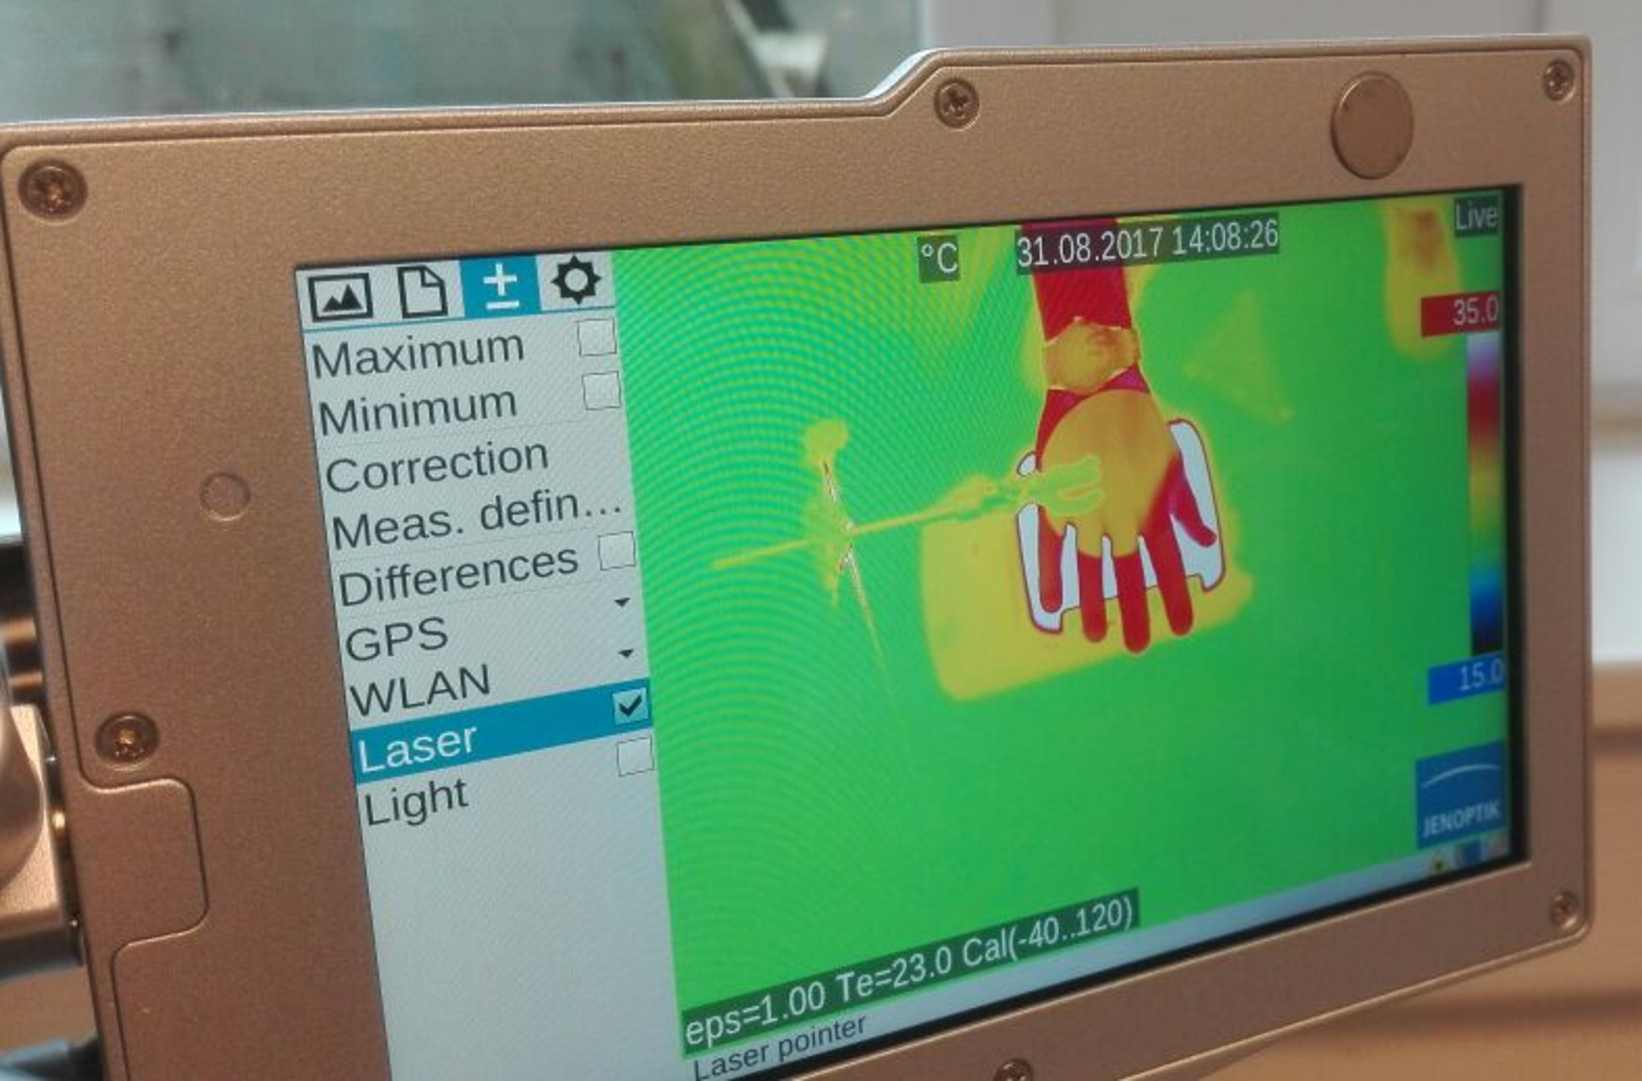
\includegraphics[scale=0.35]{Figures/Chapter04/HandTransmission.pdf}
			\caption{IR image (taken directly with the camera) of a circular piece of silicon wafer similar to the one glued on the polished side of the Petal showing the high transmissivity properties of the silicon. Behind the silicon there is a heating plate at 150\space$^\circ C$ and in between the experimenter's hand (we can clearly see the fingers shape through the silicon).}\label{fig4.4}
		\end{figure}
		
		\begin{figure}[ht!]
			\centering
			\captionsetup{justification=centering,margin=2cm}
			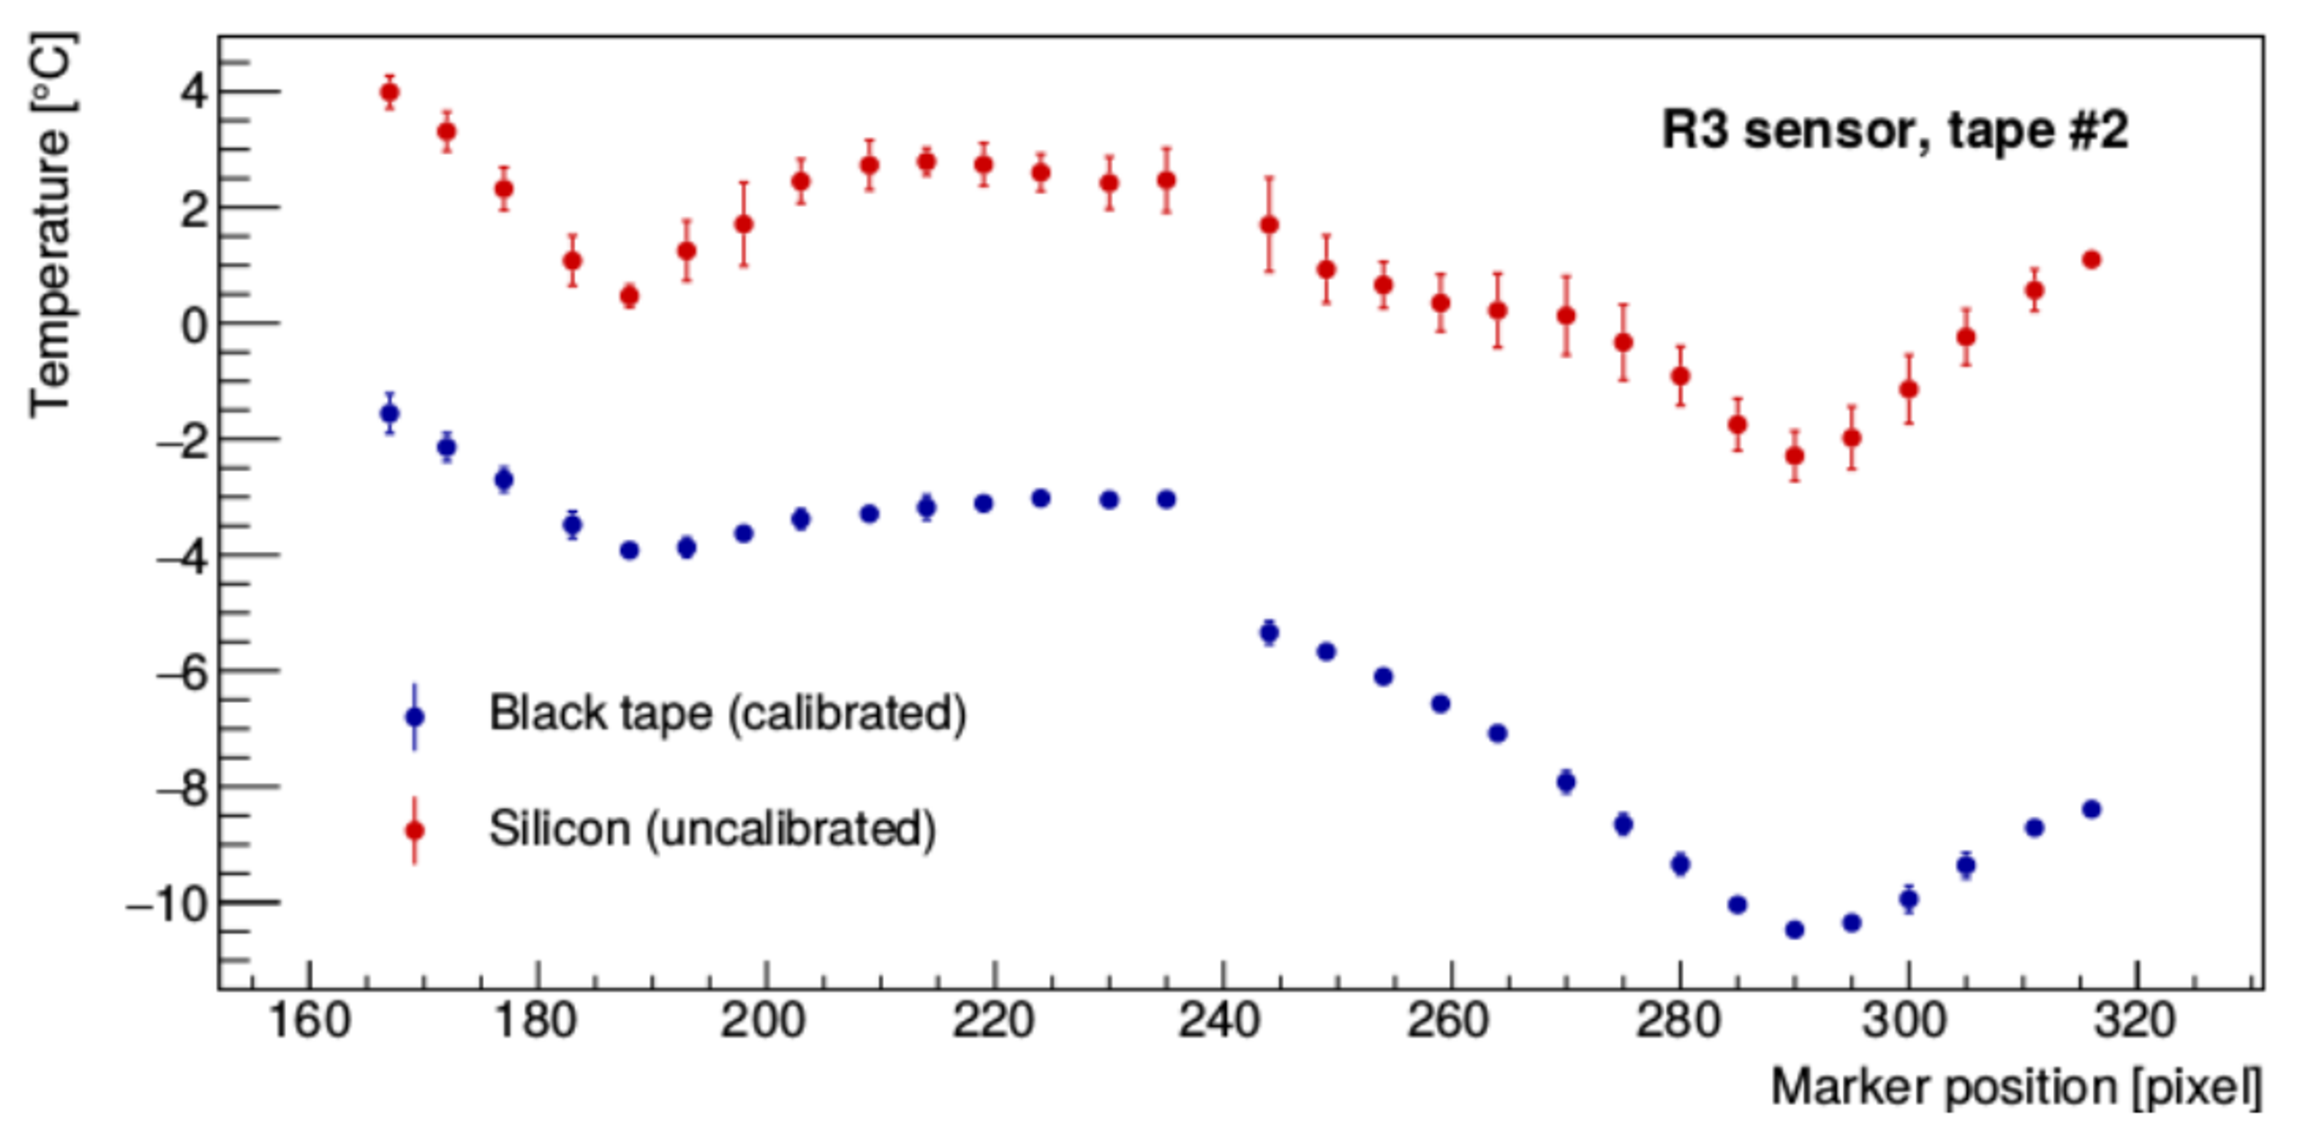
\includegraphics[scale=0.35]{Figures/Chapter04/R3Profile_Si_and_BT.pdf}
			\caption{Temperature profile plot of the second (middle) black tape strip in module R3 for the lowest temperature setpoint.}\label{fig4.5}
		\end{figure}
		
		After applying Equation \ref{eq3.14} on each pair of silicon - black tape markers and using the software emissivity calculation tool we obtained the results shown in Figure \ref{fig4.6}. As we can see the Equation \ref{eq3.14} estimations are in good agreement with the software outputs. 
		
		\begin{figure}[ht!]
			\centering
			\captionsetup{justification=centering,margin=2cm}
			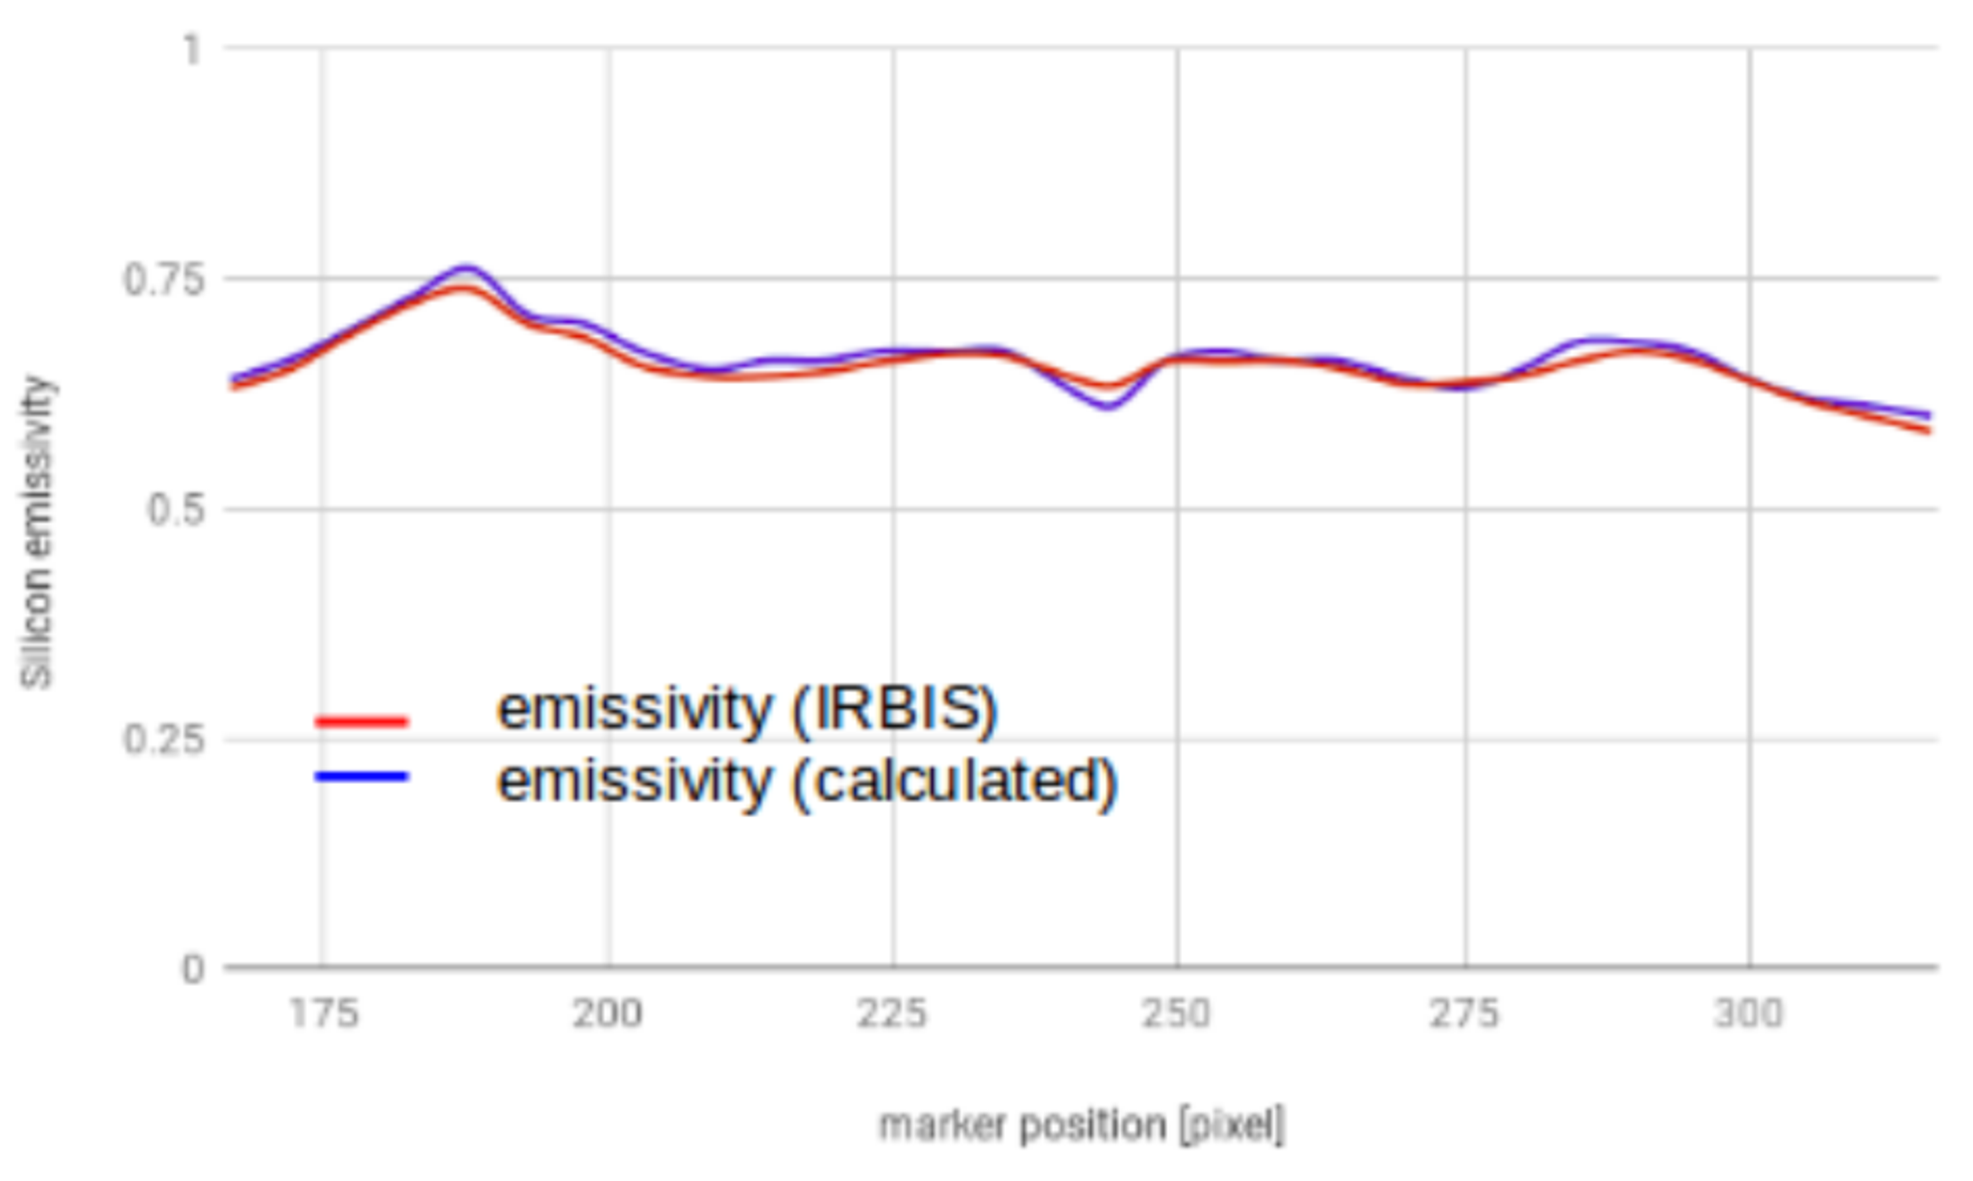
\includegraphics[scale=0.35]{Figures/Chapter04/SiliconEmissivityCalculatedVSIRBIS.pdf}
			\caption{Silicon emissivity calculated using Equation 3.14 (blue line) and the emissivity calculation tool provided by the IR camera software (red line).}\label{fig4.6}
		\end{figure}
		
		The average emissivity is estimated to be around $0.66 \pm 0.07$. By entering this value in the IRBIS software we could correct “globally” the pixels temperature to yield silicon temperatures more close to the real values. However, this would worsen the calibration for the rest of the surfaces making their temperature values to shift greatly from the truth value.
	
	\section{IR camera spectral response scale factor.}\label{section4.4}
	
		As discussed in the previous section, a global approach to the thermogram calibration can be made to obtain realistic temperature values in the silicon surface but, by doing so, we would lost valuable information about the rest of the surfaces. Evidently we would need some way to be able to correct the thermograms at pixel level. The first approach would be then to try to estimate the pixels emissivity for the entire image. In the following we will propose a methodology to estimate the pixel emissivity by means of a so called “baseline” image. 
		
		Let's assume that we have a thermogram of which we know the real temperature of all the pixels. That could be, for example, a thermogram of the Petal at room temperature. The fact that we still see differences of temperature in the image even though everything is at the same temperature (See Figure \ref{fig3.4}) is evidence (to a first approximation) of the effect of the different emissivity values of the materials composing the Petal. We call such image a baseline thermogram. The advantage of the baseline thermogram is that we know the real temperature of all the pixels beforehand and therefore we could use Equation \ref{eq3.9} to calculate the emissivity of each pixel. However, first we must determine the IR camera’s average spectral response ($R$) which we will treat in the next section. 
		This method, however, presents an associated difficulty discussed before: the baseline is at room temperature, which means that we can not use Equation \ref{eq3.9} directly to obtain emissivity but, instead, we can use it iteratively to estimate emissivity to some degree of accuracy. Of course this makes even worse the errors in the estimation of emissivity but it's the price to pay for not touching the Petal. The other important disadvantage is that, in order to be able to extrapolate the values of emissivity calculated on the baseline image to other thermograms we must be sure that the camera does not move from one to the other, otherwise the pixels won't match anymore and the emissivity values would not be valid.
		Finally, we have also assumed that the emissivity does not depend on the surface temperature under the graybody approximation, which is not true in general. However, except for the case of selective emitters, emissivity is a very slowly-variating function of the surface's temperature.
		
		\bigskip
		Figure \ref{fig4.7} (left) shows the results of the estimation of the $R$ scale factor for the IR camera. The method used was described in section \ref{section3.1.3}, however, to test the method's validity we used as well a Petal thermogram of which we knew the real surface temperatures, that is, the powered off Petal at room temperature. Figure \ref{fig4.7} (right) shows the scale factor estimation on the Petal.
		
		\begin{figure}[ht!]
			\centering
			\captionsetup{justification=centering,margin=2cm}
			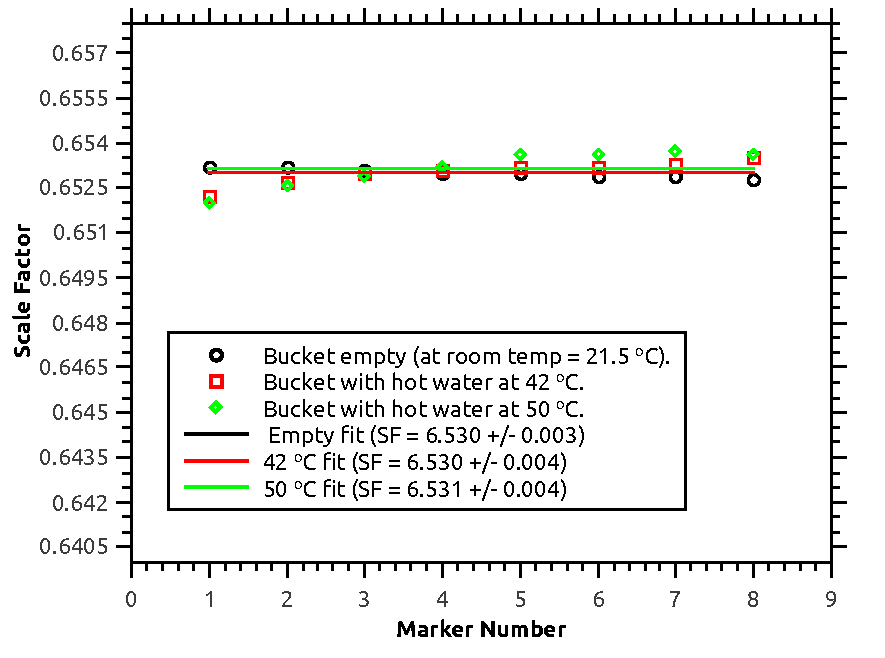
\includegraphics[scale=0.5]{Figures/Chapter04/BucketScaleFactors.pdf}
			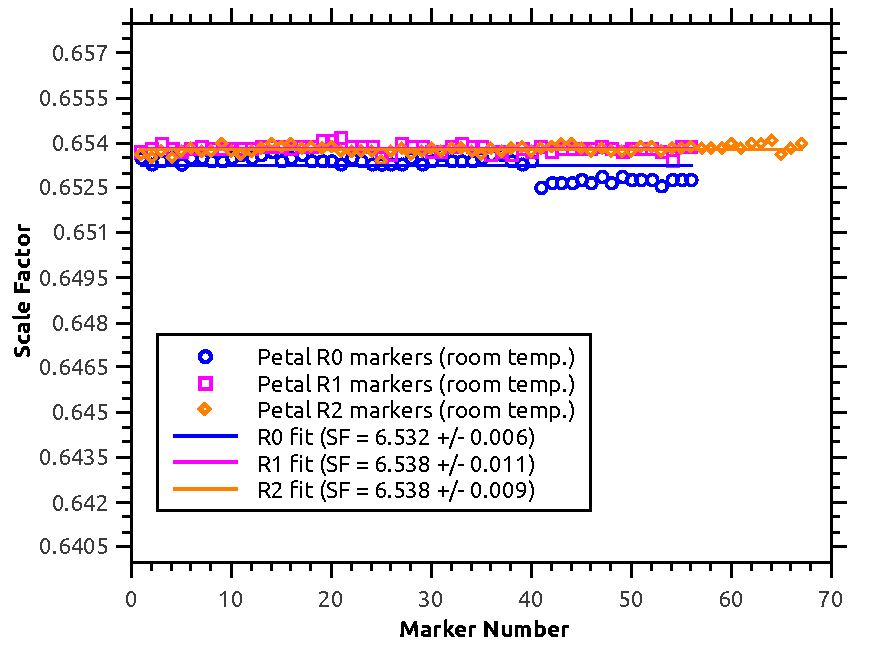
\includegraphics[scale=0.5]{Figures/Chapter04/PetalScaleFactors.pdf}
			\caption{Fits of the IR camera response scale factor calculated for different temperatures (left) and using a Petal thermogram (right).}\label{fig4.7}
		\end{figure}
		
		For the calculations, the values of the black tape in silicon modules R0, R1 and R2 were used, showing consistent results with the values obtained with the aluminum bucket. The uncertainty shown is the fit's root mean squared error. With this test we corroborated that this factor is only dependent on the IR sensor/camera and independent of the temperature and the surface.
	
	\section{Viewing angle influence in the measurements.}\label{section4.5}
	
		In order to test whether or not the viewing angle played a significant role in the IR temperature measurements, the aluminum rod filled with water at 34.6\space$^\circ C$ described in section \ref{section3.1} was used. The results can be seen in Figure \ref{fig4.8}. 
		We observed that the temperature variations along the rod are within 1\space$^\circ C$ including the error bands from an angle of 0$^\circ$ (with respect to the normal of the rod's surface) to roughly 30$^\circ$. For the central values this difference is less than 0.2\space$^\circ C$. This is a relatively small variation for that angular range and even though we see a drop in the markers temperature with respect to the real temperature (measured with a thermocouple directly inside the rod) the error magnitude make us conclude that, within this uncertainty, the angle influence on the IR temperature measurements is quite negligible.
		
		\begin{figure}[ht!]
			\centering
			\captionsetup{justification=centering,margin=0cm}
			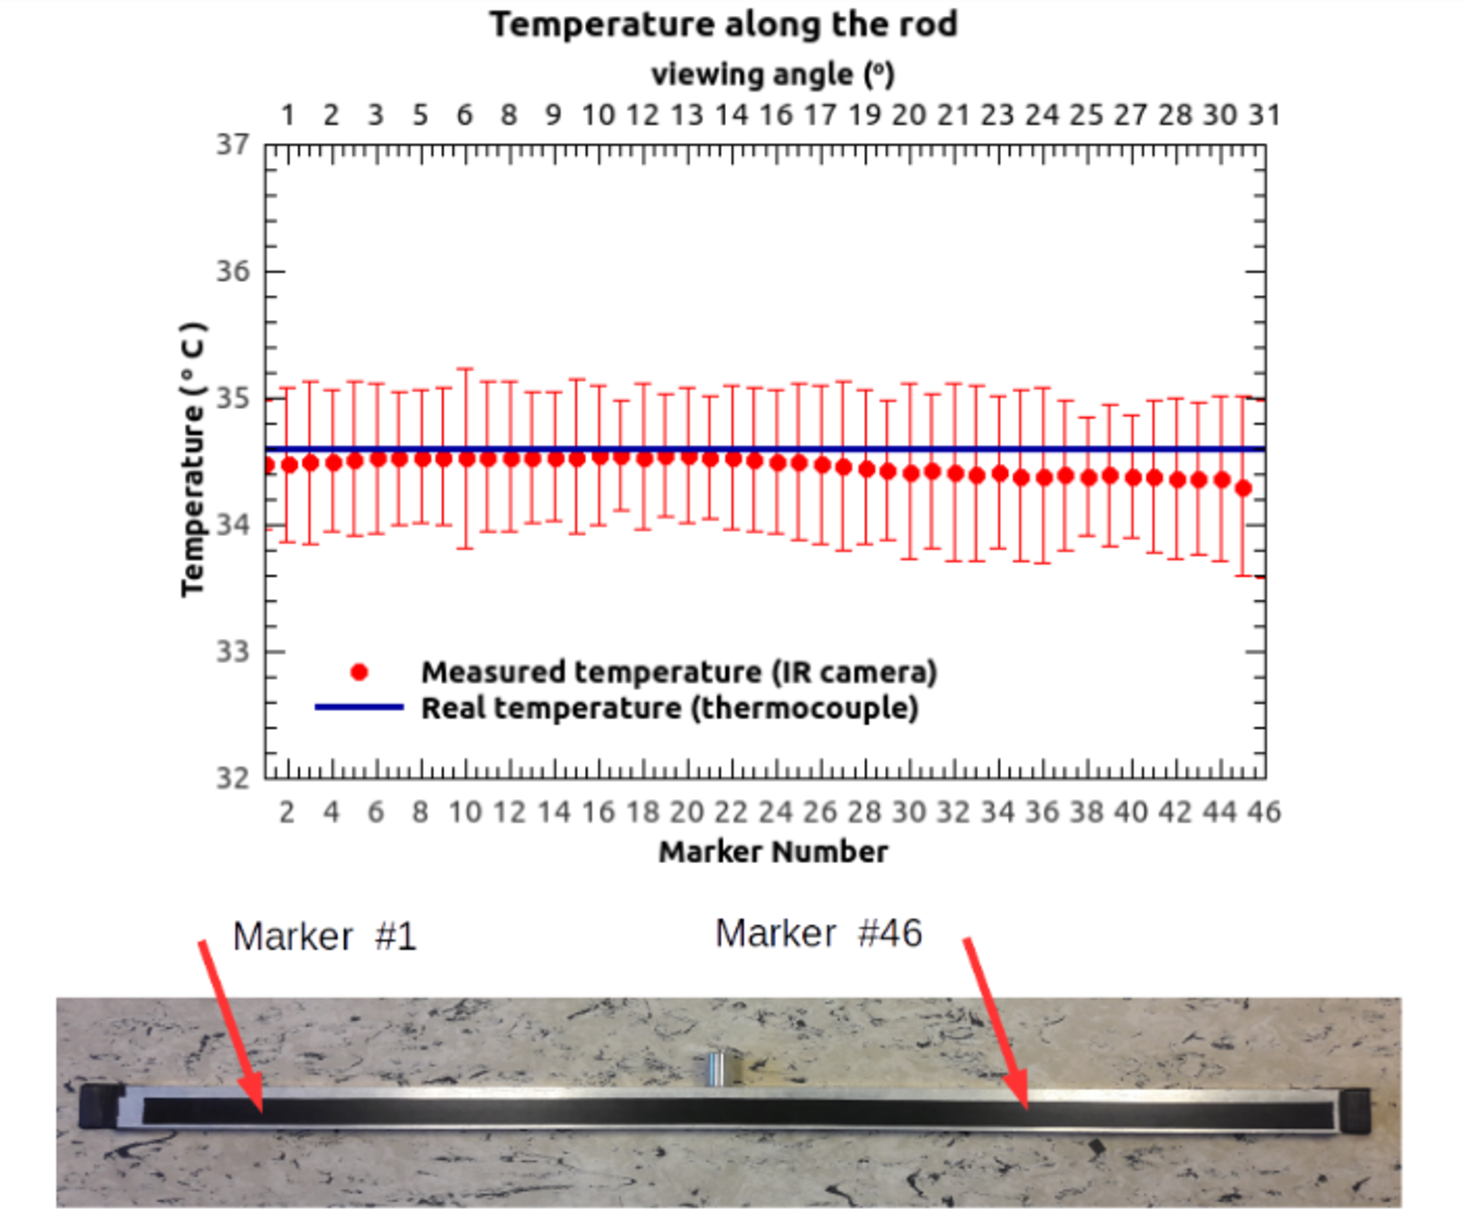
\includegraphics[scale=0.4]{Figures/Chapter04/RodAngularTempResults.pdf}
			\caption{Angle study results (top) using the aluminum rod filled with water at 34.6\space$^\circ C$ (bottom). The marker positions do not cover the entire rod since it is larger than the Petal and some portions fall out of the viewing field of the camera.}\label{fig4.8}
		\end{figure}
	